% !TEX encoding = UTF-8
%% Vorlage für LEN-Aufgaben
%% Basiert auf der KOMA-Article-Klasse
%% weiter Informationen unter http://www.komascript.de
%%
%% Bei Fragen kannst Du dich auch an die Organisatoren des LaTeX-Einfuerungs-
%% kurses der Fachschaft wenden. Du erreichst uns unter:
%% latex@fachschaft.etec.uni-karlsruhe.de
%% 
%% 2010/11/30 Ferdinand Schwenk
\documentclass[%
  a4paper, %
  12pt, %
   article, %
  titlepage
]{scrartcl}

%% Zeichensatzkodierung 
%% Unter Windows [latin1]
%% Unter Linux [utf8] verwenden.
\usepackage[utf8]{inputenc}
\usepackage[T1]{fontenc}
\usepackage[ngerman]{babel}

%% Zusatz Pakete einbinden
% Zum Einbinden von Quelltexten
\usepackage{listings}
% !TEX encoding = UTF-8
%% Definition der Quelltextformatierung
%% 
%% 2010/11/30 Ferdinand Schwenk
\lstset{%
  language=Matlab,                    % Sprache: Matlab
  numbers=left,                       % Nummerierung: links
  numberstyle=\tiny,                  % Formatierng der Nummerierung
  numbersep=8pt,                      % Abstand der Nummerierung vom Quelltext
  frame=trBL,                         % Rahmen um den Quelltext
  rulecolor=\color{blue},             % Farbe des Rahmens
  rulesepcolor=\color{red},           %
  backgroundcolor=\color[gray]{0.9},  %
  extendedchars=true,                 %
  breaklines=true,                    %
  basicstyle=\scriptsize              %
}
        % Einstellungen für das linstings-Paket laden

% Bilder und Farbe
\usepackage{graphicx}
\usepackage{color}


\setlength{\parindent}{0pt}
 \usepackage{url}

% Mathematische Formeln
\usepackage{amsmath}

% Tabellen
\usepackage{tabularx}

%% Meta-Informationen
\author{%
\raggedright
  \normalsize %
  \begin{tabularx}{\textwidth}{|l|X|}%
    \hline%
    \textbf{Vorname:}         & Niklas \\ \hline
    \textbf{Nachname:}        & Fauth \\ \hline
    \textbf{Matrikelnummer:}  & 1932872 \\ \hline
    \textbf{RZ-Account:} & UTEDE \\ \hline
    \textbf{Punkte:}          &  \\ \hline % Hier sollst DU wohl nichts eintragen ;-)
  \end{tabularx}%
}
% ------------------------------------------------------------------------------
% Die Informationen in diesem Bereich bitte nicht aendern
% !TEX encoding = UTF-8
% !TEX root = vorlage.tex
%% Erstellt die Titelseite für die LEN-Aufgaben
%% 
%% 2010/11/30 Ferdinand Schwenk
\title{Spice-Aufgabe WS 15/16}
% ------------------------------------------------------------------------------
% Die Informationen in diesem Bereich bitte nicht aendern
\titlehead{%
  \begin{tabularx}{\linewidth}{|>{\centering\arraybackslash}X|>{\centering\arraybackslash}X|}%
    \hline%
    \multicolumn{2}{|c|}{\large Karlsruher Institut f\"ur Technologie} \\
    \multicolumn{2}{|c|}{\large \textbf{Institut f\"ur Biomedizinische Technik}} \\ \hline
    Prof. Dr. rer. nat. O. D\"ossel & M. Sc. M. Kircher \\ & Dipl. Ing. J. Schmid\\
    \scriptsize Kaiserstr. 12 / Geb. 30.33 & \scriptsize Kaiserstr. 12 / Geb. 30.33 \\
    \scriptsize Tel.: 0721 / 608-42650 & \scriptsize Tel.: 0721 / 608-2751 \\
    \hline %
  \end{tabularx}%
}
\subject{Lineare Elektrische Netze}
\date{  }
\publishers{
\raggedright
\normalsize{\underline{Angaben zur Bearbeitung der Aufgaben:}\vspace{0.2cm}\\ 
Die Aufgaben m\"ussen selbstst\"andig und ohne fremde Hilfe bearbeitet werden.\vspace{0.2cm}\\
Der L\"osungsweg muss vollst\"andig angegeben und nachvollziehbar sein! Dokumentieren Sie Ihre \"Uberlegungen, geben Sie erl\"auternde Kommentare!\vspace{0.2cm}\\
Die maximale Punktzahl dieser Aufgabe entspricht 3\% der Gesamtpunktzahl der Endnote im Fach Lineare Elektrische Netze.\\
\vspace{0.8cm}
\textbf{Eidesstattliche Erkl\"arung}\\
\vspace{0.2cm}
Hiermit erkl\"are ich an Eides statt, dass ich die vorliegende
Arbeit  selb\-stst\"andig  und  ohne  unzul\"assige fremde Hilfsmittel angefertigt habe. W\"ortlich oder inhaltlich \"ubernommene Stellen sind als solche kenntlich gemacht und die verwendeten Literaturquellen im Literaturverzeichnis  vollst\"andig angegeben. Die \glqq Regeln zur Sicherung guter wissenschaftlicher Praxis im Karlsruher Institut f\"ur Technologie (KIT)\grqq\, in ihrer g\"ultigen Form wurden beachtet. \\
\vspace{1.5cm}
Karlsruhe, den \rule{10 cm}{0.4pt}
\hspace*{6cm}\footnotesize{{Datum und Unterschrift}}

}}

% ------------------------------------------------------------------------------

% ------------------------------------------------------------------------------

% Hier beginnt das Dokument
\begin{document}
  % Erstellt die Titelseite
  \maketitle

  %Gibt das Inhaltsverzeichnis aus
\begingroup
\let\cleardoublepage\clearpage
\tableofcontents

\endgroup
\bigskip 
Diese Dokumentation sowie dazugehörige Grafiken und Quellcode kann unter
\bigskip 
\\
\url{https://github.com/NiklasFauth/Private_Projects/tree/master/SPICE}
\bigskip 
\\abgerufen werden.
\clearpage
  
  %% Hier kannst du jetzt Deinen Lösungstext schrieben.
  %% Grafiken einbinden (*.pdf oder *.png):
  %%   \includegraphics{Pfad/zu/Deinem/Bild}
  %%   \includegraphics[width=BREITE,height=HOEHE,keepaspectratio]{Pfad/zu/Deinem/Bild}
  %% Quelltext einbinden:
  %%   \lstinputlisting[caption={BESCHRIFTUNG}]{Pfad/zu/deinem/quelltext}



\section{Aufgabe}
\subsection{Aufgabenteil a}
Die Dargestellte Schaltung nennt man einen nichtinvertierenden Verstärker.

\subsection{Aufgabenteil b}
Da der Operationsverstärker im linearen Bereich betrieben wird, kann angenommen werden, dass die Spannungsdifferenz zwischen den Eingängen 0V beträgt.
Da kein Strom in die Eingänge des Operationsverstärker fließ, können R1 und R2 als unbelasteter Spannungsteiler betrachtet werden.
Damit ergibt sich :

\begin{equation}
U_{a1} = U_{a} * \frac{R_{2}}{R_{1} + R_{2}} 
\end{equation}
\begin{equation}
U_{a} = U_{a1} * \frac{R_{1} + R_{2}}{R_{2}}
\end{equation}

Der Verstärkungsfaktor beträgt demnach

\begin{equation}
\frac{U_{a}}{U_{a1}} =  \frac{R_{1} + R_{2}}{R_{2}} = 10
\end{equation}

In Dezibel:

\begin{equation}
\frac{U_{a}}{U_{a1}} = 20 * log(\frac{U_{a}}{U_{a1}})dB = 20dB
\end{equation}\

\subsection{Aufgabenteil c}

Für $\omega$ = 0 ist die Impedanz der Kondensatoren unendlich hoch. Sie können damit in der Schaltung vernachlässigt werden, Schaltungsteil A reduziert sich auf eine Reihenschaltung von 
$RN_{1}$ und $RN_{2}$.

\clearpage

\subsection{Aufgabenteil d}

Nun sollte die Schaltung mittels LTSpice simuliert werden. Dazu wurden verschiedene Widerstandswerte
(RN = 51k, 68k, 85k) sowie verschiedene Frequenzen (1Hz - 1000Hz) gewählt.

\begin{figure}[h]
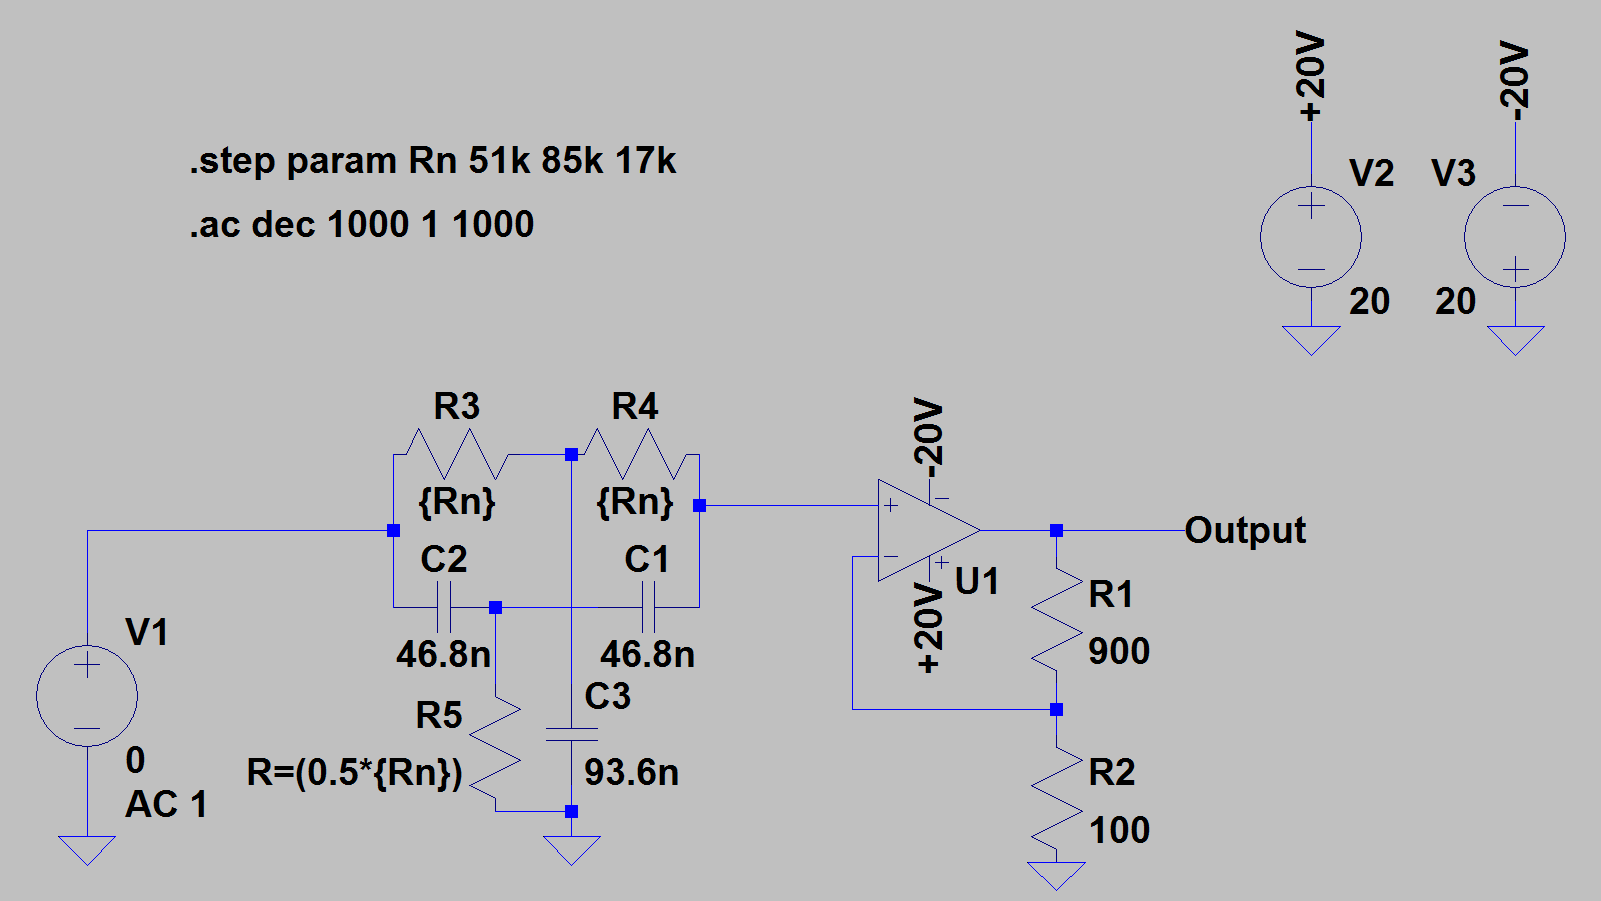
\includegraphics[width=\textwidth]{schematic2.png}
\caption{Spice-Schaltung}
\label{fig1}
\end{figure}

\clearpage

\begin{figure}[h]
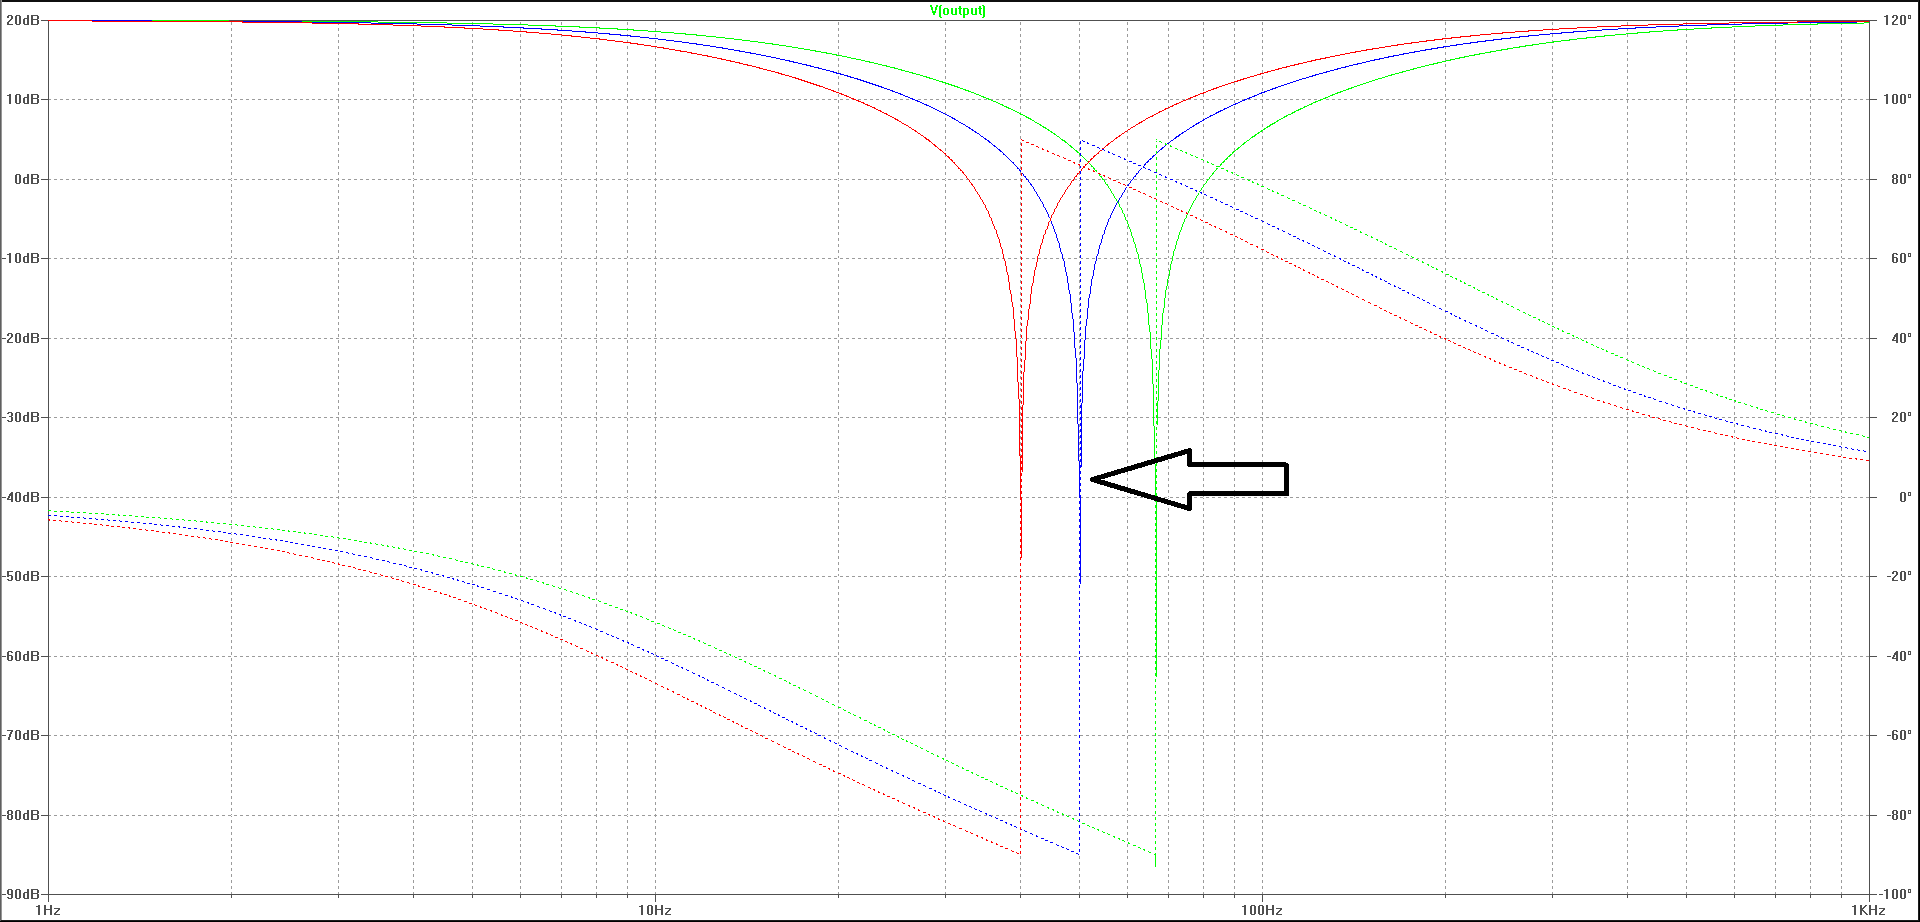
\includegraphics[width=\textwidth]{plot1.png}
\caption{Bodediagramm}
\label{fig2}
\end{figure}


\subsection{Aufgabenteil e}

Nun sollte der Widerstandswert gewählt werden, der die Störung durch die Netzfrequenz am Besten unterdrück. 
Hierzu eignet sich RN = 68k sehr gut.

\clearpage

\section{Aufgabe}
\subsection{Aufgabenteil a}

Die Impedanz der Schaltung ergibt sich aus der Reihenschaltung von R und L welche wiederum parallel zum Kondensators
C geschaltet sind. Zusätzlich muss die Reihenschaltung mit $R_{last}$ beachtet werden.

\begin{equation}
Z_{ges}=R_{Last}+\frac{(R+j\omega L)\frac{1}{j\omega C}}{R+j\omega L+\frac{1}{j\omega C}}
\end{equation}

Mit Wolfram|Alpha  kann nun der Real- und Imaginärteil bestimmt werden. (r = $R_{last}$)

\begin{figure}[h]
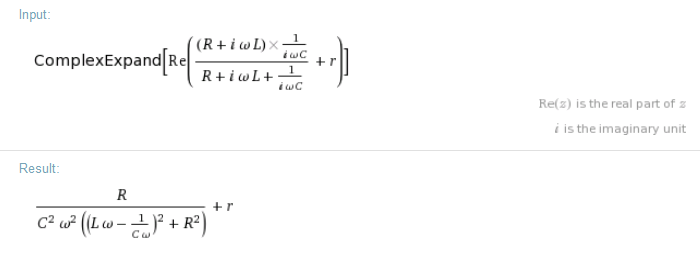
\includegraphics[width=\textwidth]{wolfram1.png}
\caption{Realteil}
\label{fig3}
\end{figure}

\begin{figure}[h]
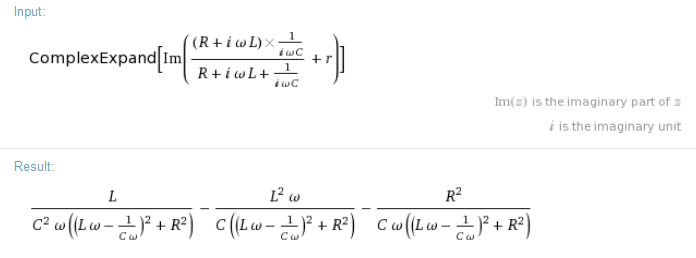
\includegraphics[width=\textwidth]{wolfram2.png}
\caption{Imaginärteil}
\label{fig4}
\end{figure}

\clearpage

\subsection{Aufgabenteil b}
Nun sollen die Frequenzen bestimmt werden, bei denen die Eingangsspannung Ue
und der Strom $I_{last}$ in Phase sind. Da hier die Impedanz vollständig reel ist, können die Nullstellen der Imaginärteils gesucht werden.

\begin{figure}[h]
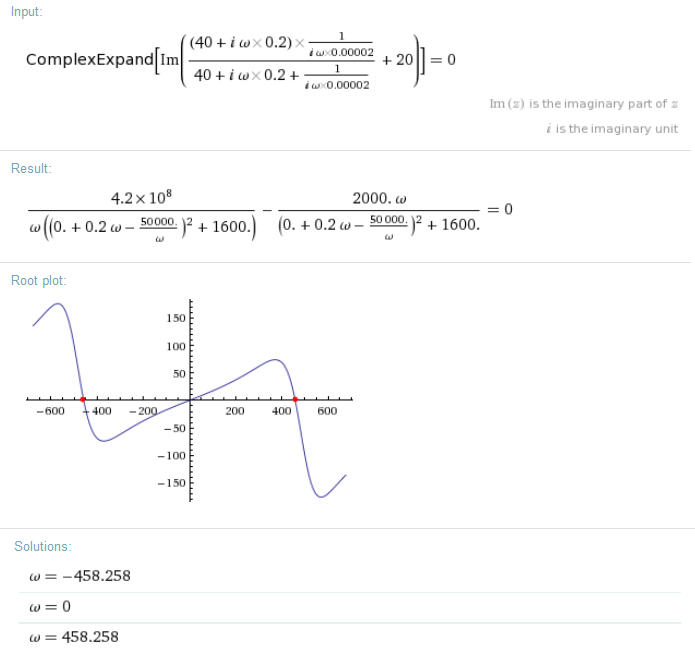
\includegraphics[width=\textwidth]{wolfram3.png}
\caption{Lösung mit Wolfram|Alpha}
\label{fig5}
\end{figure}

Natürlich kann die Frequenz nicht negativ sein. Die praktisch relevante Freqnez beträgt demnach f = 72,934Hz.









\end{document}